\documentclass[a4paper]{article}
\usepackage[utf8x]{inputenc}
\usepackage[lastexercise]{exercise}
\usepackage{color}
\usepackage[absolute]{textpos} 
\usepackage{verbatim}
\usepackage{tikz}
\usetikzlibrary{calc}
\usetikzlibrary{positioning}

\renewcommand\ExerciseName{Exercice}
\renewcommand{\AnswerHeader}{\medskip\centerline{\textbf{Solution de
                        l'\ExerciseName  \ExerciseHeaderNB}\smallskip}}
\newenvironment{CAnswer}{\color{red}\begin{Answer}}
                        {\end{Answer}}

\title{Prolog - TP3}
\date{}

\begin{document}
\maketitle
\begin{textblock*}{4cm}(10mm,10mm)
\begin{Large}ESIAL 3A IL LE\end{Large}
\end{textblock*}
\begin{textblock*}{3cm}(160mm,10mm)

\includegraphics[width=\textwidth]{../../ESIAL.pdf}
\end{textblock*}

\begin{Exercise}[title={la coupure (sur feuille)}]
Soit le programme suivant :
\begin{verbatim}
s(a). (1)
s(b). (2)
t(a,b). (3)
t(b,a). (4)
p1(X,Y):- s(X),t(Y,X). (5)
p1(a,a). (6)

p2(X,Y):- s(X),t(Y,X),!. (7)
p2(a,a). (8)

p3(X,Y):- s(X),!,t(Y,X). (9)
p3(a,a). (10)

p4(X,Y):- !,s(X),t(Y,X). (11)
p4(a,a). (12)
\end{verbatim}

Quel est l'arbre de recherche prolog à la question \verb#p1(X,Y)#,
\verb#p2(X,Y)#, \verb#p3(X,Y)# et \verb#p4(x,y)# ?
\end{Exercise}
\begin{CAnswer}
\begin{center}
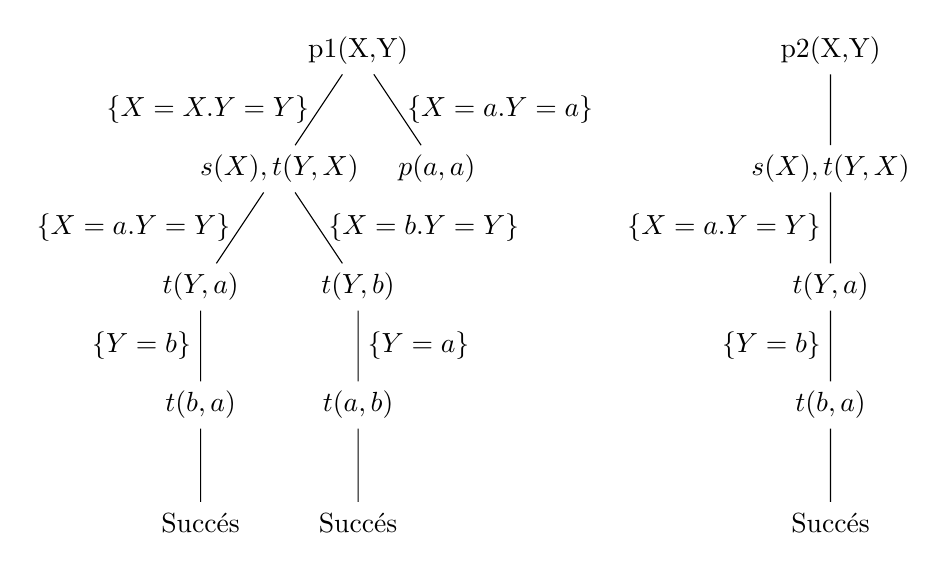
\begin{tikzpicture}[nodes={minimum size=1.5em},
                    level 1/.style={sibling distance=20mm}]
 \node {p1(X,Y)} 
   child {node {$s(X),t(Y,X)$} 
           child {node {$t(Y,a)$}
                   child {node {$t(b,a)$}
                           child {node {Succ\'es}}
                           edge from parent 
                                node[left] {$\{Y=b\}$} 
                         }
                   edge from parent 
                        node[left] {$\{X=a. Y=Y\}$} 
                 }
           child {node {$t(Y,b)$}
                   child {node {$t(a,b)$}
                           child {node {Succ\'es}}
                           edge from parent 
                                node[right] {$\{Y=a\}$} 
                         }
                   edge from parent 
                        node[right] {$\{X=b. Y=Y\}$} 
                 }
           edge from parent 
                node[left] {$\{X=X. Y=Y\}$} 
         }
   child {node {$p(a,a)$}
           edge from parent 
                node[right] {$\{X=a. Y=a\}$}
         };
 \node at (6,0) {p2(X,Y)} 
   child {node {$s(X),t(Y,X)$} 
           child {node {$t(Y,a)$}
                   child {node {$t(b,a)$}
                           child {node {Succ\'es}}
                           edge from parent 
                                node[left] {$\{Y=b\}$} 
                         }
                   edge from parent 
                        node[left] {$\{X=a. Y=Y\}$} 
                 }
         };
\end{tikzpicture}
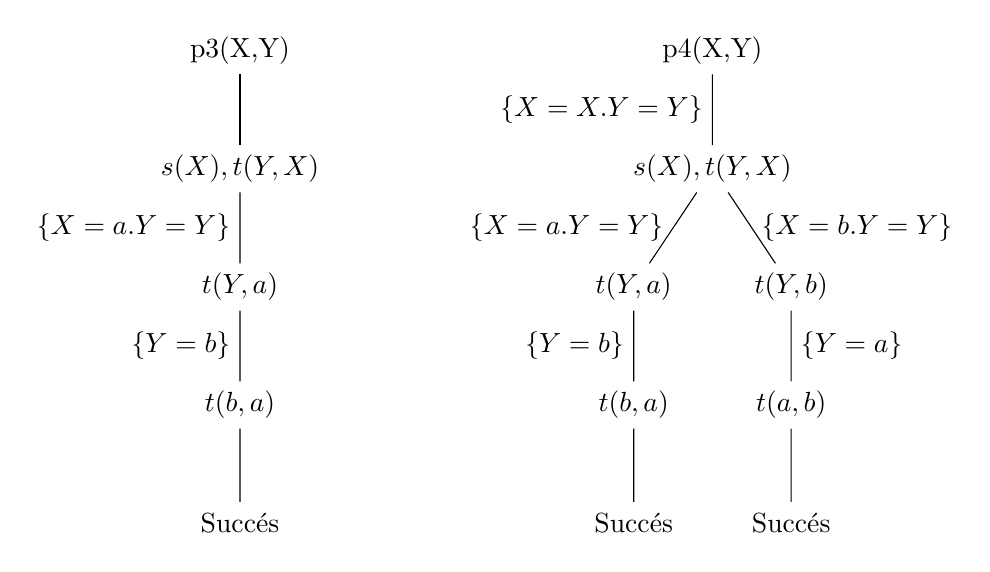
\begin{tikzpicture}[nodes={minimum size=1.5em},
                    level 1/.style={sibling distance=20mm}]
 \node {p3(X,Y)} 
   child {node {$s(X),t(Y,X)$} 
           child {node {$t(Y,a)$}
                   child {node {$t(b,a)$}
                           child {node {Succ\'es}}
                           edge from parent 
                                node[left] {$\{Y=b\}$} 
                         }
                   edge from parent 
                        node[left] {$\{X=a. Y=Y\}$} 
                 }
         };
 \node at (6,0) {p4(X,Y)} 
   child {node {$s(X),t(Y,X)$} 
           child {node {$t(Y,a)$}
                   child {node {$t(b,a)$}
                           child {node {Succ\'es}}
                           edge from parent 
                                node[left] {$\{Y=b\}$} 
                         }
                   edge from parent 
                        node[left] {$\{X=a. Y=Y\}$} 
                 }
           child {node {$t(Y,b)$}
                   child {node {$t(a,b)$}
                           child {node {Succ\'es}}
                           edge from parent 
                                node[right] {$\{Y=a\}$} 
                         }
                   edge from parent 
                        node[right] {$\{X=b. Y=Y\}$} 
                 }
           edge from parent 
                node[left] {$\{X=X. Y=Y\}$} 
         };
\end{tikzpicture}
\end{center}
\end{CAnswer}

\begin{Exercise}[title={calcul du maximum}]
Commencez par recopiez le programme suivant :
\begin{verbatim}
max1(X,Y,Z):- X >= Y.
max1(X,Y,Y):- X < Y.

max2(X,Y,X):- X >= Y, !.
max2(X,Y,Y):- X < Y.

max3(X,Y,X):- X >= Y,!.
max3(X,Y,Y).
\end{verbatim}

Comprenez comment fonctionne ces prédicats et vérifiez leur comportement.
Voici quelques exemples que vous pouvez utiliser :
\begin{verbatim}
max*(1,2,X).
max*(4,2,X).
max*(4,2,2).
\end{verbatim}

Quel est le problème de max3 ? Ecrivez un nouveau prédicat max4 qui corrige
ce problème (indice : utilisez \verb#=/2# )
\end{Exercise}
\begin{CAnswer}
\subparagraph{Avec max1 :}
\begin{verbatim}
| ?- max1(1,2,X). 
X = 2 

| ?- max1(4,2,X). 
X = 4 ;
no (tente la deuxième clause du prédicat)

| ?- max1(4,2,2). 
no 
\end{verbatim}

\subparagraph{Avec max2 :}
\begin{verbatim}
| ?- max2(1,2,X). 
X = 2 
yes 

| ?- max2(4,2,X). 
X = 4 
yes (ne tente plus la deuxième clause du prédicat grâce à la coupure)

| ?- max2(4,2,2). 
no 
\end{verbatim}

\subparagraph{Avec max3 :}
\begin{verbatim}
| ?- max3(1,2,X). 
X = 2 
yes 

| ?- max3(4,2,X). 
X = 4 
yes 

| ?- max3(4,2,2). 
yes 
\end{verbatim}
Ce dernier prédicat ne marche pas quand la variable de  résultat  est
instanciée. En effet l'unification avec la première clause ne marche pas
car on a 4 différent de 2 et la deuxième clause marche toujours

\subparagraph{Correction du problème :}
Pour garder la deuxième clause identique, il faut pouvoir forcer la 
vérification de l'inégalité. Pour cela on n'unifie pas tout de suite X avec
le résultat.
\begin{verbatim}
max4(X,Y,Z):- X >= Y,!, Z = X.
max4(X,Y,Y).
\end{verbatim}
\end{CAnswer}


\begin{Exercise}[title={insérer un élément dans une liste}]
Ecrivez un prédicat \verb#insérer/3# qui permet d'insérer un entier dans une 
liste triée par ordre croissant. Vous ferez en sorte que ce prédicat soit 
déterministe.
\begin{verbatim}
| ?- inserer(3,[],X).   
X = [3] 
yes 

| ?- inserer(3,[2,4],X). 
X = [2,3,4] 
yes 

| ?- inserer(3,[4,5],X). 
X = [3,4,5] 
yes 
\end{verbatim}
\end{Exercise}
\begin{CAnswer}
\verbatiminput{inserer.pro}
\end{CAnswer}


\begin{Exercise}[title={inversion d'une liste}]
Au cours du TP 2, vous avez écrit le prédicat \verb#inverser/2# qui permet
d'inverser une liste. Ecrivez un nouveau prédicat permettant d'inverser une
liste en utilisant un accumulateur et un wrapper.
\begin{verbatim}
?­ inverse([a,b,c,d], [d,c,b,a]). 
yes 
\end{verbatim}
\end{Exercise}
\begin{CAnswer}
\begin{verbatim}
inverse(L,R):­  accInv(L,[],R). 
accInv([T|Q],A,R) :­  accInv(Q,[T|A],R). 
accInv([],A,A). 
\end{verbatim} 
\end{CAnswer}


\begin{Exercise}[title={nombre d'occurrences d'un terme}]
Ecrivez un prédicat \verb#occurrence/3#. \verb#occurrence(X,Liste,N)# compte
le nombre \verb#N# d'éléments de la liste déjà identique à \verb#X#. Cela
signifie que ce prédicat est d'un niveau métalogique car Prolog ne doit pas
essayer d'unifier les termes au risque de rajouter de termes identiques.

Appuyez vous sur les exemples suivants pour bien comprendre :\\
Juste :
\begin{verbatim}
| ?- occurrence(a,[a,b,c,X,a,a],N). 
N = 3 
yes 
\end{verbatim}
Faux :
\begin{verbatim}
| ?- occurrence2(a,[a,b,c,X,a,a],N). 
N = 4 
X = a 
yes 
\end{verbatim}

Dans ce cas Prolog a unifié \verb#X# avec a alors qu'en fait nous on veut
compter les termes déjà identiques\\
Juste :
\begin{verbatim}
| ?- occurrence(X,[a,b,c,X,a,a],N). 
N = 1 
yes 
\end{verbatim}
Faux : 
\begin{verbatim}
| ?- occurrence2(X,[a,b,c,X,a,a],N). 
N = 4 
X = a 
\end{verbatim}
Cet exemple montre bien que l'on veut compter le nombre de terme \verb#X# dans
la liste et cela sans l'instancier au préalable.
\end{Exercise}
\begin{CAnswer}
\verbatiminput{occurence.pro}
\end{CAnswer}


\begin{Exercise}[title={les dérivées}]
Le but de cet exercice est de calculer formellement les dérivées d'une 
fonction. Rappelez vous qu'en Prolog les expressions arithmétiques sont
déjà représentées comme des structures.

Vous vous baserez sur les transformations suivantes. On considère $x$ comme
paramètre de la fonction, $*$ représente la multiplication et $c$ une
constante.\\
\begin{math}
c' \rightarrow 0\\
x' \rightarrow 1\\
(-U)' \rightarrow -(U')\\
(U + V)' \rightarrow U' + V'\\
(U – V)' \rightarrow U' – V'\\
(c * U)' \rightarrow c * U'\\
(U * V)' \rightarrow U * V' + V * U'\\
(U /  V)' \rightarrow (UV-1)'\\
(Uc)' \rightarrow c U-1 U'
\end{math}

L'opérateur exposant est représenté en prolog par \verb#**/2# :
\begin{verbatim}
| ?- X is 3**3.                 
X = 27.0 
yes 
\end{verbatim}

Ecrivez le prédicat \verb#derive(E,X,R)# qui réussit quand \verb#R# est la
dérivée de l'expression \verb#E# avec comme paramètre \verb#X#. On considérera
que les deux premiers paramètres sont instanciées et que le dernier est une
variable (le résultat de la dérivée).
 
Voici quelques exemples :
\begin{verbatim}
| ?- derive(x**2+2*x+1,x,X).    
X = 2*x**(2-1)*1+2*1+0 
yes 

| ?- derive(-x/2,x,X). 
X = -1*2**(-1-1)*0* -x+ - 1*2** -1 
yes 

| ?- derive(3*x**2+x**2+1+3/(x**2),x,X).    
X = 3*(2*x**(2-1)*1)+2*x**(2-1)*1+0+3*(-1*(x**2)**(-1-1)*(2*x**(2-1)*1)) 
yes 
\end{verbatim}
Vous pouvez ensuite définir un prédicat \verb#simp(E1,E2)# qui à partir d'une
expression \verb#E1# instanciée calcule \verb#E2# qui est une forme simplifiée.
Il faut considérer 2 cas :
\begin{itemize}
 \item on ne peut pas simplifier car on n'a pas de terme composé
 \item on peut simplifier car on un terme avec un opérateur et deux arguments
\end{itemize}
Ce deuxième cas peut être traité par un prédicat annexe \verb#change/4#.
\verb#change(op,gauche,droit,E)# réussit avec \verb#E# l'expression simplifiée
de l'expression 'gauche op droit'. Ce prédicat peut être construit de manière
incrémentale. Commencez par exemple par traiter le cas 0 + Y = Y. Complétez
ensuite les différents cas de l'addition puis les cas de la multiplication.
\end{Exercise}
\begin{CAnswer}
\verbatiminput{derive.pro}
\end{CAnswer}


\begin{Exercise}[title={Tic-Tac-Toe }]
Cet exercice traite du fameux jeu du Tic-Tac-Toe (Morpion). Nous n'allons pas
créer un programme entier qui permettrait de jouer contre une IA mais seulement
un programme d'aide à la décision très basique. 

Le jeu se compose d'une grille de 9 cases numérotées comme ci-dessous :
\begin{center}
\begin{tabular}{|c|c|c|}\hline
 1 & 2 & 3 \\\hline
 4 & 5 & 6 \\\hline
 7 & 8 & 9 \\\hline
\end{tabular}
\end{center}

Le jeu se joue à deux joueurs jouant à tour de rôle:
\begin{itemize}
 \item le premier peut écrire un 'x' dans une case
 \item le second peut écrire un 'o' dans une case
\end{itemize}

L'objectif est d'aligner trois 'x' ou 'o' pour gagner.

Créez un programme permettant d'aider le joueur avec les 'o' dont le but est
de lui indiquer quelle case jouer dans le cas où il est certain qu'il perde au
prochain coup s'il ne joue pas cette case.

Nous considérerons le plateau comme une structure : 
\verb#plateau(C1,C2,C3,C4,C5,C6,C7,C8,C9)#

\verb#Ci# représente la case $i$ de la grille. \verb#Ci# est soit une variable
non instanciée (case non jouée) ou un 'x' ou un 'o'.

Cet exercice est un cas classique d'un programme qui génère et teste. Il faut
donc faire en sorte de générer les différents cas à vérifier (c'est à dire où
le joueur risque de perdre) puis de vérifier si le joueur risque vraiment de
perdre dans ce cas.

Vous pouvez utiliser les prédicats \verb#arg/3#, \verb#var/1# et
\verb#nonvar/1# pour accéder aux cases du plateau et examiner leur contenu.

Créez un prédicat \verb#mouvement_obligatoire/2# tel que 
\verb#mouvement_obligatoire(Plateau,X)# retourne le numéro de la case à jouer
en fonction du plateau de jeu courant.

On veut obtenir :
\begin{verbatim}
| ?- mouvement_obligatoire(prateau(C1,C2,C3,C4,C5,C6,C7,C8,C9),X). 
no 

| ?- mouvement_obligatoire(plateau(x,C2,C3,C4,x,o,o,C8,C9),X).    
X = 9 
yes 
\end{verbatim}
\begin{center}
\begin{tabular}{|c|c|c|}\hline
 x &   &   \\\hline
   & x & o \\\hline
 o &   & !!! \\\hline
\end{tabular}
\end{center}
\end{Exercise}
\begin{CAnswer}
\verbatiminput{tictactoe.pro}
\end{CAnswer}
\end{document}
